\documentclass[twoside, 12pt, a4paper]{article}
%\include{IAP_References.bib}
% List Of Packages
\usepackage{geometry, graphicx, color, fancyhdr, setspace, caption, url}
\usepackage{psfrag,amsbsy,amsmath,textcomp,enumerate}
\usepackage[font=footnotesize]{caption}
\usepackage[nottoc,numbib]{tocbibind}
\usepackage[hidelinks]{hyperref}
\usepackage{multirow}
\usepackage{makecell}
\usepackage{float}
\usepackage{setspace}
\usepackage{notoccite}
\usepackage{longtable}
\usepackage{lscape}
\usepackage{siunitx}
\usepackage{subcaption}
\usepackage{pdflscape}
\usepackage{booktabs}
\usepackage{multicol}
\usepackage{textgreek}

%\graphicspath{ {./Lab2_Images_Reformatted/} }
%\usepackage{natbib}
% Define Use Of Packages
% Geometry
\geometry{margin = 2.5cm}
\newenvironment{where}{\noindent{}where\begin{itemize}}{\end{itemize}}
\renewcommand{\refname}{REFERENCES}
\renewcommand{\contentsname}{TABLE OF CONTENTS}
%\renewcommand{\listfigurename}{LIST OF FIGURES}
%\renewcommand{\listtablename}{LIST OF TABLES}
% Enter Information
\newenvironment{myindentpar}[1]%
{\begin{list}{}%
		{\setlength{\leftmargin}{#1}}%
		\item[]%
	}
	{\end{list}}

% Fancyhdr
\pagestyle{fancy}
\fancyhead[R]{3803ICT Big Data Analysis, 2022}
\fancyhead[L]{}
\fancyfoot[LE,RO]{\thepage}
\fancyfoot[LO]{Jessy Barber}       % put your names here for fancy footer
\fancyfoot[RE]{Your Title}            % put title here for fancy header
\fancyfoot[C]{}
\renewcommand{\footrulewidth}{0.4pt}

%\bibliographystyle{IEEE}

% Begin The Document
\begin{document}
\begin{titlepage}
\begin{flushright}
	
\includegraphics[height=60px]{griffithlogo.png}
\end{flushright}
\begin{large}
\textbf{Griffith School of Information and Communication Technology}\\
\textbf{Griffith University}

\vspace*{8mm}

\textbf{3803ICT - Big Data Analysis}\\
\textbf{Trimester 1, 2022}
\end{large}

\vspace*{15mm}

\begin{Huge}
\begin{center}
\textbf{Lab Report:}\\
\textbf{Job Market Analysis}
\end{center}
\end{Huge}

\vspace*{5mm}
\begin{large}


\vspace*{8mm}

\textbf{Jessy Barber, s5138877}\\
\newline

\vspace*{8mm}
\begin{myindentpar}{2cm}
\emph{A report submitted in partial fulfilment of the degree of Bachelor of Electrical Engineering (Honours) / Bachelor of Computer Science}
\end{myindentpar}



\end{large}


\vfill

\end{titlepage}
%-----------------------------------------------------------------------------------------

%next four lines create blank page
%\pagebreak
%\pagestyle{empty}
%\textcolor{white}{This is a blank page}
%\pagebreak

% Contents page

\pagestyle{fancy}
\fancyfoot[C]{\thepage}
\fancyfoot[L,R]{}
\pagenumbering{roman}
\setcounter{page}{1}


%\cleardoublepage
%\phantomsection 

% ----------------------------------------------------------------
\tableofcontents


%\listoffigures
%\listoftables

% ----------------------------------------------------------------
%Document content goes here.
\newpage
\pagenumbering{arabic}
\setcounter{page}{1}
\pagestyle{fancy}

\fancyfoot[LE,RO]{\thepage}
\fancyfoot[LO]{Jessy Barber, s5138877}                    % insert names for footer here
\fancyfoot[C]{}

\section{Data Preparation and Preprocessing}
The data used in this exploratory analysis will be the provided excel spread sheet, "data.csv". 
\subsection{Describe the Dataset}

\begin{figure}[h]
	\centering
	\includegraphics[scale = 0.65]{cats.png}
	\caption{Categories / Domains of the Dataset}
	\label{fig:cats}
\end{figure}

As seen in figure \ref{fig:cats}, the categories / domains of the dataset are clearly shown. Figure \ref{fig:cats} also shows the number of non-null values that exist in each of these categories. The types of these categories are int64, which represents the lowest salary / highest salary categories, datetime64, which has been used to convert the Date category from its original object format, and the rest of the data are object file formats. The object file format represent strings since these categories contain strings describing their respective job meta data. The original job market dataset contains 13 columns of categories and contains 318'477 rows.\\
This report will conduct multiple vectors of analysis on this job data including analysis on the job metadata / attributes, analysis on the market by locations and analysis on the market by sectors. This analysis will then be visualised using an interactive visualiser. For the attribute analysis, the sector / sub-sectors for each job will be studied, along with the location and range of salaries for each job. The locational analysis will take a further look at the market size in each city and their hottest sectors. The range of salaries common in each city and where the employees are best paid will also be studied. Additionally, the pattern of job posts for each city will be analysed. The market's sectors will then be studied to determine which sectors keep the highest market share, which sub-sectors are of particular interest, what salary ranges are common for each sector / sub-sector, what is the market trend in terms of its sectors and which skills are required for each sector. 

\newpage
\subsection{Describe the Steps You Used for Data Preparation and Preprocessing}

The data is loaded using pandas as per the following code:

\begin{figure}[h]
	\centering
	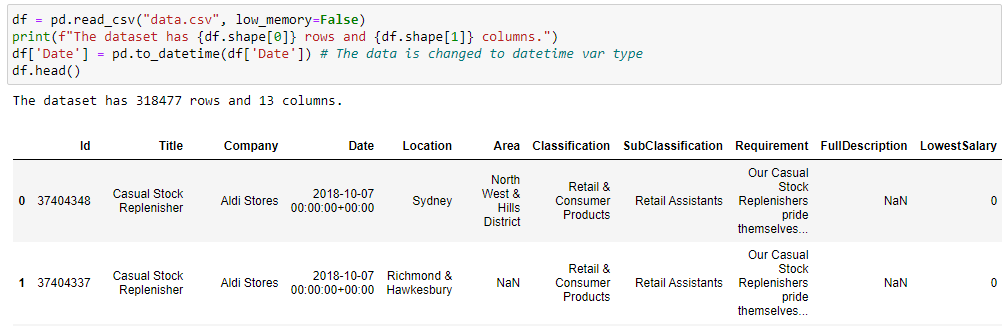
\includegraphics[scale = 0.60]{LoadingDataCode.png}
	\caption{Loading the Data with Pandas}
	\label{fig:LoadingData}
\end{figure}

As seen in figure \ref{fig:LoadingData}, the .csv file is read in and stored as a DataFrame type in the variable df. The head of the dataframe is then printed for visualisation purposes. 

HOW DO YOU NORMALISE THE DATA:\\
HOW DO YOU CLEAN THE DATA:

\subsection{Hypothesis About the Analysis Outcome}

\newpage 
\section{Data Analysis and Interpretation}
%This section involves performing exploratory analysis, performing statistical analysis and performing predictive analysis on the job market dataset. 
\subsection{Studying the Job Meta Data / Attributes}

\begin{figure}[h]
	\centering
	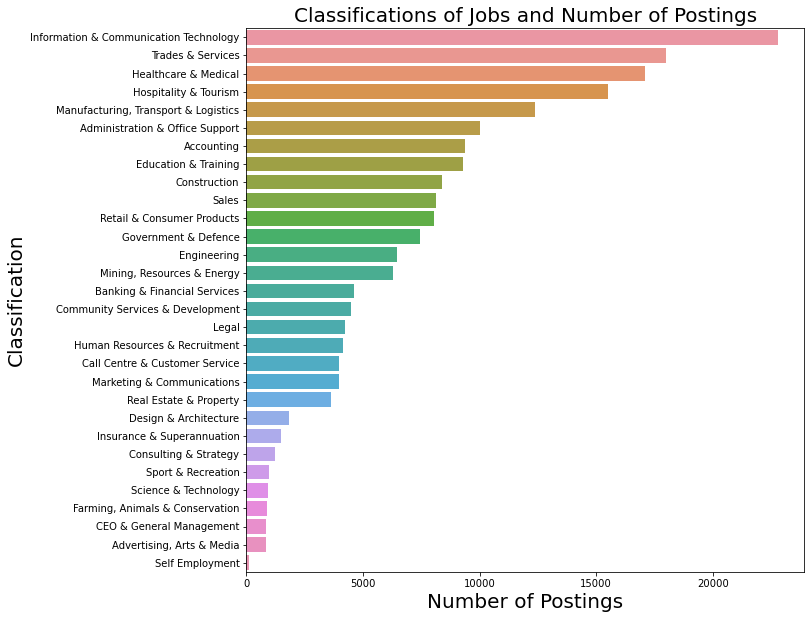
\includegraphics[scale = 0.45]{ClassVsPostings.png}
	\caption{Classification of Jobs and Number of Postings}
	\label{fig:ClassVsPosts}
\end{figure}

\begin{figure}[h!]
	\centering
	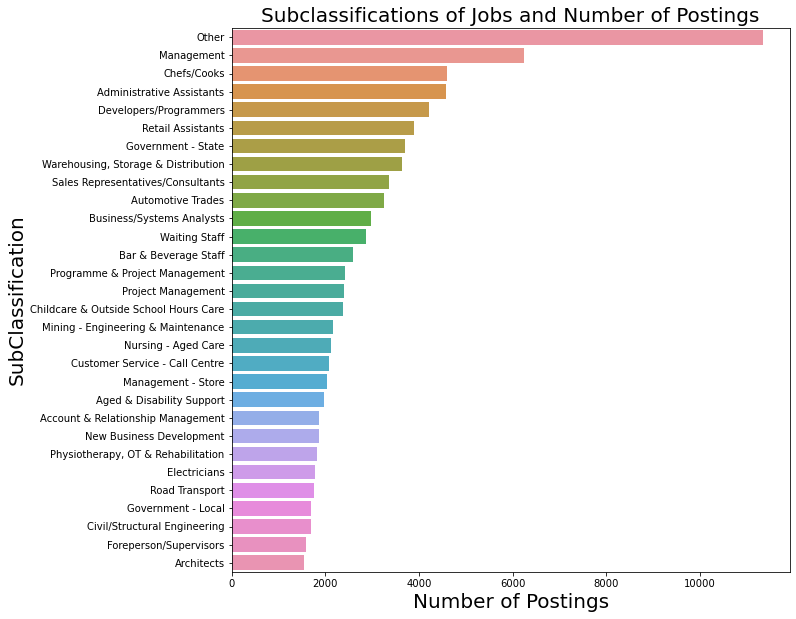
\includegraphics[scale = 0.45]{SubClassVsPostings.png}
	\caption{Subclassification of Jobs and Number of Postings}
	\label{fig:SubClassVsPosts}
\end{figure}

\newpage 
Figure \ref{fig:ClassVsPosts} shows the 30 unique job classifications from the market dataset. Figure \ref{fig:ClassVsPosts} also shows the posting frequency of each of these classifications with information and communication technology, trades and services, healthcare and medical, hospitality and tourism and manufacturing, transport and logistics being in the top five.\\\\
Figure \ref{fig:SubClassVsPosts} shows the top 30 sub classifications from the market dataset. Figure \ref{fig:SubClassVsPosts} also shows the posting frequency of each of these sub classifications with other, management, chefs / cooks, administrative assistants and developers / programmers being in the top five. 

\begin{figure}[h!]
	\centering
	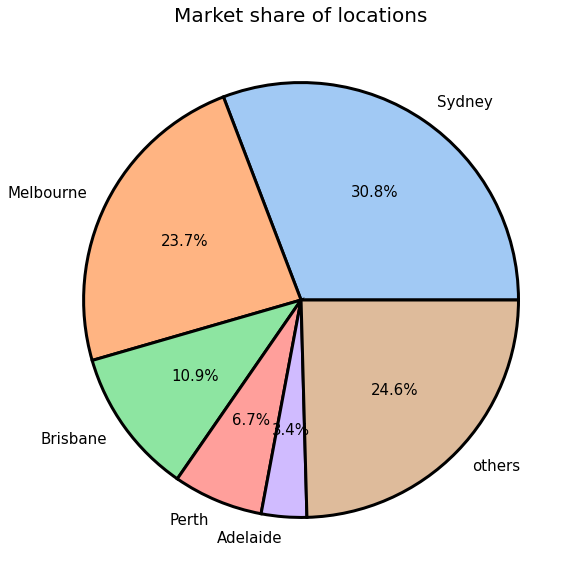
\includegraphics[scale = 0.58]{TopCities.png}
	\caption{Top Five Cities for Market Share}
	\label{fig:TopFiveCities}
\end{figure}

Figure \ref{fig:TopFiveCities} shows the top five cities in Australia in terms of market share from the dataset. It is clear that Sydney holds the highest market share of employment at 30.8\% and Melbourne in second with 23.7\% of the market share. Adelaide presents the lowest market share at 3.4\%. 

\newpage
\begin{figure}[h!]
	\centering
	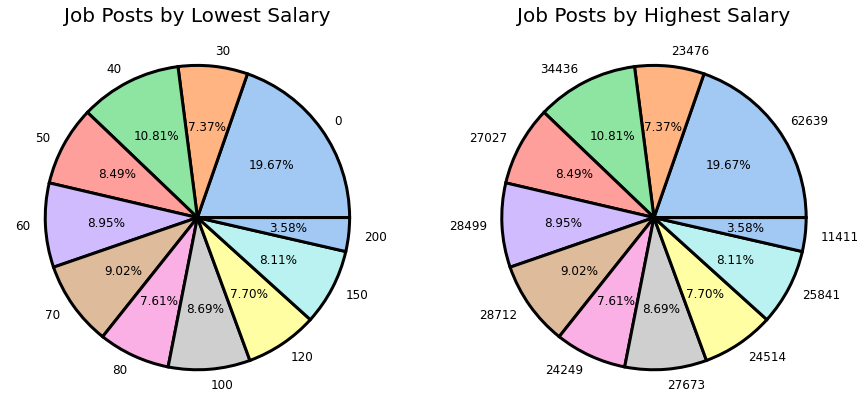
\includegraphics[scale = 0.55]{SalaryRanges.png}
	\caption{Salary Ranges of Jobs}
	\label{fig:SalaryRanges}
\end{figure}

Figure \ref{fig:SalaryRanges} shows the highest and lowest salary ranges for each job. WHAT DOES 0 REPRESENT -> UNEMPLOYMENT OR NAN. TALK ABOUT TOP LOWEST AND TOP HIGHEST SALARIES. 



\end{document}
